\documentclass[12pt,a4paper]{report}
\usepackage[latin1]{inputenc}
\usepackage{amsmath}
\usepackage{amsfonts}
\usepackage{subfigure}
\usepackage{amssymb}
\usepackage[pdftex]{graphicx}
\begin{document}

Note that filter groups are the horizontal neighbors in all plots. All pooling was with no overlap.  

\begin{figure}[h]
\centering
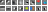
\includegraphics[scale=5]{L2_f2s1.png}
\caption{$L_2$ pooling across features only (groups of 2) }
\end{figure} 

\begin{figure}[h]
\centering
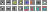
\includegraphics[scale=5]{max_weak_f2s2.png}
\caption{Max pooling across features and space (groups of 2, 4 spatial neighbors). Weak slowness penalty. }
\end{figure} 

\begin{figure}[h]
\centering
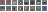
\includegraphics[scale=5]{max_strong_f2s2.png}
\caption{Max pooling across features and space (groups of 2, 4 spatial neighbors). Strong slowness penalty. }
\end{figure} 

\begin{figure}[h]
\centering
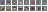
\includegraphics[scale=5]{max_f2s4.png}
\caption{Max pooling across features and space (groups of 2, 16 spatial neighbors). Note the weak group association when the spatial neighborhood is increased.}
\end{figure} 

\begin{figure}[h]
\centering
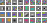
\includegraphics[scale=5]{large.png}
\caption{ \emph{Training in progress, has not converged yet.} Max pooling across features and space (groups of 2, 4 spatial neighbors).}
\end{figure} 

\begin{figure}[h]
\centering
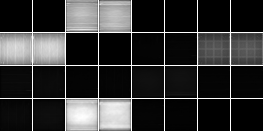
\includegraphics[scale=1]{large_act.png}
\caption{ \emph{Training in progress, has not converged yet.} Activations averaged over the dataset for the filters above. I think 'plaid patterns' are due to compression artifacts in the images that it picks up on. Note that, by far the most popular features are local low-pass followed by horizontal and vertical edges.}
\end{figure} 


\end{document} 